%---------------------------------------------------------------------------------
%*****************************************************
% This main.tex is written by D.CHIBOUTI
% I wish you enjoy !!!
%*****************************************************
%---------------------------------------------------------------------------------
\documentclass{DChibouti}

%---------------------------------------------------------------
%---------------------------------------------------------------
%---------------------------------------------------------------
%%%%%%%%%%%%%%%% PAGE DE GARDE %%%%%%%%%%%%%%%%
%---------------------------------------------------------------
%------------------------------------------------------------
%---------------------------------------------------------------
\title{Titre de votre stage ou votre TP}

\lesoustitre{Le sous titre}

\discipline{Compte rendu TP ou stage de Master MFT}

\author{D. Chibouti}

\date{\today}

\nomdeuniversite{Université Gustave Eiffel}
\logouniversite{img/logo_Gustave} %nom du fichier
\scalelogouniversite{0.4} % mise a l'echelle de l'image (0.5=50% par exemple)
\logolabo{img/logo_MSME}
\scalelogolabo{0.75}
%---------------------------------------------------------------
%------------------------------------------------------------
%---------------------------------------------------------------




\makeindex


\makenomenclature
% -----------------------------------------
%% This code creates the groups
% -----------------------------------------
\usepackage{etoolbox}
\renewcommand\nomgroup[1]{%
  \item[\bfseries
  \ifstrequal{#1}{A}{Abréviation}{%
  \ifstrequal{#1}{C}{Constantes}{%
  \ifstrequal{#1}{G}{Symboles Physiques}{%
  \ifstrequal{#1}{N}{Number Sets}{%
  \ifstrequal{#1}{P}{Paramètres Numériques}{%
  \ifstrequal{#1}{R}{Grandeurs Physiques en Grecque}{}}}}}}%
]}
% -----------------------------------------






\begin{document}
%page de garde
\maketitle  % soit avec make title ou bien on inclut lapage de garde directement
%\include{page_de_garde}  %essayez la 

\clearpage
%\include{none}
\vspace*{0.05\textheight}
% % \chapter*{Remerciements}
\begin{center} 
\Huge\textbf{Remerciements} 
\end{center}
\thispagestyle{empty}

\vspace*{0.05\textheight}

Je tiens tout d’abord à remercier ...

\vspace*{0.03\textheight}
J'adresse également toute ma reconnaissance à ...

\vspace*{0.03\textheight}
J’exprime également ma gratitude à ...
\vspace*{0.03\textheight}
Enfin, ces remerciements ...

\vspace*{0.05\textheight}
\noindent\enquote{\itshape Les rêves ne peuvent pas devenir réalité... Les objectifs, bien au contraire, se réalisent si on persiste... Il faut de la persévérance, du courage et de la volonté}
\bigbreak
\hfill D. CHIBOUTI


\newpage
\vspace*{0.05\textheight}

\begin{center} 
\Huge\textbf{Résumé} 
\end{center}

La simulation moléculaire ...
\vskip 1 cm
\textbf{Mots clés} : Dynamique Moléculaire, Fortran/MPI ... 

 
\begin{center} 
\Huge\textbf{Abstract} 
\end{center} 

\textbf{Computing of the heat flux near a fluid-solid interface using "Molecular Dynamics"}
\vskip 0.3 cm
Molecular simulation is ...
\vskip 1 cm
\textbf{Keywords}: Molecular Dynamics, Fortran/MPI ...
 

\tableofcontents
\listoffigures
\listoftables
\makenomenclature
\clearpage


%%%%%%%%%%%%%%%%%%%%%%%%%%%%%%%%%%%%%%%%%%%%%%%%%%%%%%%%%%%%%
%----------------------------------------------------------------------------------------
%	NOMENCLATURE
%----------------------------------------------------------------------------------------
\markboth{NOMENCLATURE}{NOMENCLATURE}
\addcontentsline{toc}{chapter}{Nomenclature}
% ----------------------------------------

% ----------------------------------------
% Grandeurs Physiques G
% ----------------------------------------
% ----------------------------------------
%\scriptsize
{{\footnotesize{\nomenclature[P]{$g$}{Constante de gravité}
\nomenclature[G]{$m$}{Masse}
\nomenclature[G]{$\vec f$}{vecteur force}
\nomenclature[G]{$\vec v$}{vecteur vitesse}
\nomenclature[G]{$\vec a$}{vecteur accélération}
\nomenclature[G]{$\vec r$}{vecteur position}
\nomenclature[G]{$t$}{Temps}
\nomenclature[G]{$U$}{Potentiel}
% ----------------------------------------
% Constantes en Romain R
% ----------------------------------------
% ----------------------------------------
\nomenclature[R]{$\delta t$}{Pas de temps}
% ----------------------------------------
% Constantes C
% ----------------------------------------
\nomenclature[C]{$k_{B}$}{Constante de Boltzmann ~~~~~~~~~~~~~~~~~~~~~~~$k_B~= 1.3807 \times 10^{-23} ~J/K$}
}}
% ----------------------------------------
\printnomenclature}
%%%%%%%%%%%%%%%%%%%%%%%%%%%%%%%%%%%%%%%%%%%%%%%%%%%%%%%%%%%%%


%----------------------------------------------------------------------------------------
%	SECTION 1
%----------------------------------------------------------------------------------------
\chapter*{Introduction}
\markboth{INTRODUCTION}{INTRODUCTION}
\addcontentsline{toc}{chapter}{Introduction}

Quam ob rem vita quidem talis fuit vel fortuna vel gloria, ut nihil posset accedere, moriendi autem sensum celeritas abstulit; quo de genere mortis difficile dictu est; quid homines suspicentur, videtis; hoc vere tamen licet dicere, P. Scipioni ex multis diebus, quos in vita celeberrimos laetissimosque viderit, illum diem clarissimum fuisse, cum senatu dimisso domum reductus ad vesperum est a patribus conscriptis, populo Romano, sociis et Latinis, pridie quam excessit e vita, ut ex tam alto dignitatis gradu ad superos videatur deos potius quam ad inferos pervenisse.

Le chapitre I, ...

Dans le chapitre II, ...
...
Pour finir, nous concluons sur les résultats et les perspectives envisagées.

%%%%%%%%%%%%%%%%%%%%%%%%%%%%%%%%%%%%%%%%%%%%%%%%%%%%%%%%%%%%%%%%%%%%%%%%%%%%%%%%%%%%%%%%%%%%%%%%%%%%%%%%%%%%%%%%%%%%
%----------------------------------------------------------------------------
%	CHAPTER 1
%----------------------------------------------------------------------------
\chapter{Titre du chapitre 1}

%--------------------------------------------------------------------------------
%	SECTION 1
%--------------------------------------------------------------------------------
\section{Première section}

Votre paragraphe............. Elle s’appuie sur les lois de la dynamique classique de Newton Eq. \eqref{Newton}.
%----------------------
\begin{equation}
\label{Newton}
\begin{aligned}
 m_i \ \vec {a}_i &=\vec {f}_i \\ 
 m_i \ \vec {a}_i & = m \frac{\mathrm{d} \vec {v}_i}{\mathrm{dt}}=m_i \frac{\mathrm{d}^{2} \vec {r}_i}{\mathrm{dt}^{2}}\\
 \vec {f}_i &= - \frac{\partial U}{\partial \vec {r}_i}\\
\end{aligned}
\end{equation}	   
%----------------------

où $\vec {r}_i$, $\vec {v}_i$ et $\vec {a}_i$ respectivement les vecteurs position, vitesse et accélération de la particule $i$, $m_i$ sa masse, $\vec {f}_i$ la force qu'elle subie par l'ensemble des particules qui l'entoure, $U$ représente l'énergie intermoléculaire totale entre les molécules dont l'expression sera donnée par la suite.


%%%%%%%%%%%%%%%%%%%%%%%%%%%%%%%%%%%%%%%%%%%%%%%%%%%%%%%%%%%%%%%%
%--------------------------------------------------------------------------------
%	SUB-SECTION 1-1
%--------------------------------------------------------------------------------
\subsection{Sous section de la première section}
Un texte avec une citation de l'article par exemple  \cite{CHIBOUTI2020}. 
%----------------------
\begin{figure}[htbp]
    \centering
    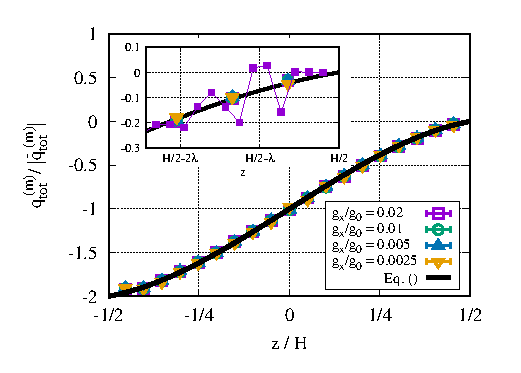
\includegraphics[scale=0.99]{img/profiles_q.eps}
    \scaption{titre de la figure}
    \label{fig:periodic}
\end{figure}
%----------------------

la figure \ref{fig:periodic} montre ........... 
%%%%%%%%%%%%%%%%%%%%%%%%%%%%%%%%%%%%%%%%%%%%%%%%%%%%%%%%%%%%%%%%
%%%%%%%%%%%%%%%%%%%%%%%%%%%%%%

%--------------------------------------------------------------------------------
%	CHAPTER 2
%--------------------------------------------------------------------------------
\chapter{Titre du Chapitre 2}
Une petite introduction à ce chapitre
%--------------------------------------------------------------------------------
%	SECTION 1
%--------------------------------------------------------------------------------
\section{Section 1}

%--------------------------------------------------------------------------------
%	SUB-SECTION 2-1
%--------------------------------------------------------------------------------
\subsection{Sous section1}

Texte pour la première sous section

%--------------------------------------------------------------------------------
%%%%%%%%%%%%%%%%%%%%%%%%%%%%%%
%--------------------------------------------------------------------------------
%	SECTION 2
%--------------------------------------------------------------------------------

\subsection{Sous section 2}
Texte pour la deuxième sous section

La table \ref{tab:tableau1} montre 
%--------------------------------------------------------------------------------
% Tableau des résultats
%--------------------------------------------------------------------------------
 \begin{table}[htbp]
	\centering
	{\small {\begin{tabular}{|ccccc|}
		\hline
		$\rho ^*$ & $A^2$  & $B_{*}$  & $C_{ref}$ & Erreur \% \\
		\hline
	    1
		& 2
		& 3
		& 4 
		& 5 $\%$\\
		0 
		& 6
		& 7
		& 8
		& 9 $\%$ \\
		\hline
		
		\end{tabular}}}
	 \scaption{Titre de la table $C_{ref}$ référence par exemple \cite{CHIBOUTI2020}}
    \label{tab:tableau1}
 \end{table}
%--------------------------------------------------------------------------------

%------------------------------------------------------------------------------------
%	SECTION FINALE
%------------------------------------------------------------------------------------

\chapter*{Conclusion}
\markboth{CONCLUSION}{CONCLUSION}
\addcontentsline{toc}{chapter}{Conclusion}


Trois volets ont été abordés durant ce travail :
\begin{enumerate}
    \item Développement de ............
    \item Validation de ...........
    \item Calcul de ........  et validation des résultats en se référant à la littérature .....  par exemple \cite{TheArt}.
\end{enumerate}

Ces différents travaux nous ont permis de tirer des conclusions 

Tout d’abord, 

De plus, ......... Ceci est d’autant plus vrai que l'erreur minimale est de l'ordre de 1\% à des temps très long et avec plusieurs échantillons.

Au cours de ce travail, nous avons mis en évidence deux points importants concernant
........ Le premier point concerne ....... En effet, en termes de ..... A l’inverse, ....

Nous pouvons donc en conclure que ..... 



En perspectives, ...
%*****************************************************


%*****************************************************
%*****************************************************
%*****************************************************


\bibliographystyle{abbrv}
\bibliography{biblio}
\addcontentsline{toc}{chapter}{Références}
\markboth{R\'EF\'ERENCES}{R\'EF\'ERENCES}


%%%%%%%%%%%%%%%%%%%%%%%%%%%%%%%%%%%%%%%%%%%%%%%%%%%%%%%
%%%%%%%%%%%%%%%%%%%%%%%%%%%%%%%%%%%%%%%%%%%%%%%%%%%%%%%
\end{document}

